\documentclass[a4paper,10pt]{book}

\usepackage{color}
\usepackage{bm}
\usepackage{amsmath}
\usepackage{appendix}
\usepackage{xspace}
\usepackage{a4wide}
\usepackage{wrapfig}
\usepackage[numbers,comma,sort&compress]{natbib}
\usepackage{graphicx}
%\usepackage{xstring}
\usepackage{listings,xcolor,courier}
%\usepackage{draftcopy}
\usepackage{longtable}
\usepackage{paralist}
%\usepackage{fancyvrb}
\usepackage{listings}

\usepackage
[dvips, %or dvips or pdftex
pagebackref, %or backref
colorlinks=true,
linkcolor=webgreen, %defined below
filecolor=webbrown, %defined below
citecolor=webgreen, %defined below
pdftitle={VOTCA-CT manual},
pdfauthor={},
pdfsubject={VOTCA-CT},
pdfkeywords={charge transport organic semiconductors},
bookmarksopen=false,
pdfpagemode=UseNone]{hyperref}

\definecolor{webgreen}{rgb}{0,.5,0}
\definecolor{webbrown}{rgb}{.6,0,0}
\pdfcompresslevel=9

\usepackage[T1]{fontenc}
%\usepackage{times}
\usepackage{type1cm}

\def\bibsection{%
    \section*{References}%
}

\begin{document}

\newcommand{\equ}[1]{eq.~\eqref{equ:#1}}
\newcommand{\Equ}[1]{Eq.~\eqref{equ:#1}}
\newcommand{\fig}[1]{figure~\ref{fig:#1}}
\newcommand{\Fig}[1]{Figure~\ref{fig:#1}}
\newcommand{\sect}[1]{section~\ref{sec:#1}}

\newcommand{\slink}[2]{\hyperref[sec:#1]{#2}}


\newcommand{\xml}{XML\xspace}
\newcommand{\gromacs}{GROMACS\xspace}
\newcommand{\gaussian}{GAUSSIAN\xspace}
\newcommand{\turbomole}{TURBOMOLE\xspace}
\newcommand{\tinker}{TINKER\xspace}

\newcommand{\Alq}{$\mathrm{Alq}_3$\xspace}
\newcommand{\dcvt}{DCV2T\xspace}

\newcommand{\xyz}{\texttt{geometry.xyz}\xspace}
\newcommand{\orb}{\texttt{zindo.orb}\xspace}
\newcommand{\votcactp}{{\MakeUppercase{votca-ctp}}\xspace}

\newcommand{\calculator}{\hyperref[sec:calculators]{calculator}\xspace}

\newcommand{\xmloptions}{\texttt{options.xml}\xspace}
\newcommand{\xmlcsg}{\texttt{map.xml}\xspace}
\newcommand{\xmlsegments}{\texttt{segments.xml}\xspace}
\newcommand{\sqlstate}{\texttt{state.db}\xspace}
\newcommand{\topology}{\texttt{topol.tpr}\xspace}
\newcommand{\trajectory}{\texttt{traj.xtc}\xspace}

\newcommand{\opt}{\texttt{{ -}-opt}\xspace}
\newcommand{\seg}{\texttt{{ -}-s}\xspace}
\newcommand{\sql}{\texttt{{ -}-db}\xspace}
\newcommand{\exe}{\texttt{{ -}-exec}\xspace}
\newcommand{\tpl}{\texttt{{ -}-top}\xspace}
\newcommand{\csg}{\texttt{{ -}-cg}\xspace}
\newcommand{\trj}{\texttt{{ -}-trj}\xspace}


\newcommand{\refcalc}{\hyperref[ref:calculators]{calculators}\xspace}

\newcommand{\overlap}{\hyperref[prog:moo_overlap]{\texttt{moo\_overlap}}\xspace}
\newcommand{\ctprun}{\hyperref[prog:ctp_run]{\texttt{ctp\_run}}\xspace}
\newcommand{\ctpmap}{\hyperref[prog:ctp_map]{\texttt{ctp\_map}}\xspace}

\newcommand{\ecoulomb}{\hyperref[calc:ecoulomb]{\texttt{ecoulomb}}\xspace}
\newcommand{\dumptraj}{\hyperref[calc:dumptraj]{\texttt{dumptraj}}\xspace}
\newcommand{\integrals}{\hyperref[calc:integrals]{\texttt{integrals}}\xspace}

\newcommand{\suggestion}[1]{{\color{red}SUGGESTION: #1}}

\newcommand{\segmentref}[1]{segments.#1}
\newcommand{\segmentopt}[1]{\hyperlink{\segmentref{#1}}{\StrSubstitute{#1}{_}{\_}}\xspace}
\newcommand{\calcref}[1]{#1}
\newcommand{\calcopt}[1]{\hyperlink{\calcref{#1}}{\StrSubstitute{#1}{_}{\_}}\xspace}

\newcommand{\calc}[1]{\hyperref[calc:#1]{\texttt{#1}}\xspace}



\frontmatter
\begin{titlepage}

%\center{\fontsize{4cm}{5cm}\selectfont VOTCA-CT}
%\center{\fontsize{1.5cm}{3cm}\selectfont USER MANUAL}

\center{\huge \sc VOTCA-CTP \\ \vspace*{1cm} Charge Transport Simulations}
\vspace*{1cm}
\center{\Large \sc User Manual}

\vspace*{3cm}
\center{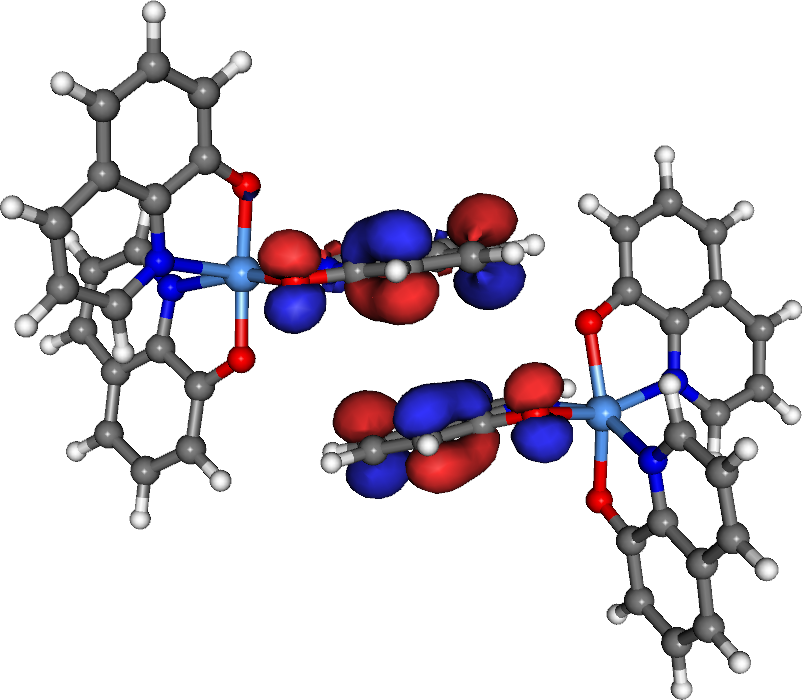
\includegraphics[width=0.6\columnwidth]{fig/logo}}
\vspace*{1cm}
\vfill

\center{\footnotesize{compiled from: \hgid}}
%\center{\footnotesize{Programs version: \refhgid}}
%\vspace*{1cm}
%\center{
%\large{\copyright \hspace*{0.1cm} VOTCA development team}
%}
\vspace*{0.5cm}
\center{\large{\today}} \\
\vspace*{0.3cm}
\htmladdnormallink{\color{black}\large{www.votca.org}}{http://www.votca.org}
\end{titlepage}

\section*{Disclamer}
The best way to start using the software is to look at provided tutorials. The reference section is generated automatically from the source code, so please make sure that your software and manual versions match.  

\section*{Citations}
Development of this software depends on academic research grants. If you are using the package, please cite the  following papers \\

\vspace{0.1cm}
\noindent
\cite{poelking_long-range_2016} Long-range embedding of molecular ions and excitations in a polarizable molecular environment, \\
Carl Poelking and Denis Andrienko \\
\htmladdnormallink{  {\itshape J. Chem. Theory Comp.} 12, 4516-4523, 2016}
{http://dx.doi.org/10.1021/acs.jctc.6b00599} \\

\vspace{0.1cm}
\noindent
\cite{ruhle_microscopic_2011} Microscopic simulations of charge transport in disordered organic semiconductors, \\
Victor R\"uhle, Alexander Lukyanov, Falk May, Manuel Schrader, Thorsten Vehoff, James Kirkpatrick, Bj\"orn Baumeier and Denis Andrienko \\
\htmladdnormallink{  {\itshape J. Chem. Theor. Comp.} 7, 3335, 2011}
{http://dx.doi.org/10.1021/ct200388s} \\

\vspace{0.1cm}
\noindent
\cite{ruhle_versatile_2009} Versatile Object-oriented Toolkit for Coarse-graining Applications \\
Victor R\"uhle, Christoph Junghans, Alexander Lukyanov, Kurt Kremer and Denis Andrienko \\
\htmladdnormallink{  {\itshape J. Chem. Theor. Comp.} 5, 3211, 2009}
{http://dx.doi.org/10.1021/ct900369w}

\section*{Development}
The core development is currently taking place at the Max Planck Institute for Polymer Research, Mainz, Germany.

\section*{Copyright}
\votcactp is free software. The entire package is available under the Apache License. For details, check
the LICENSE file in the source code. The \votcactp source code is available on our homepage, \htmladdnormallink{\color{black}www.votca.org}{http://www.votca.org}.

\vfill

\thispagestyle{empty}
\cleardoublepage

\tableofcontents
\cleardoublepage
\mainmatter
\chapter{Introduction}
\label{sec:introduction}

Charge carrier dynamics in an organic semiconductor can often be described in terms of charge hopping between localized states. The hopping rates depend on \slink{sec:transfer_integrals}{electronic coupling elements}, \slink{sec:reorganization}{reorganization energies}, and \slink{sec:site_energies}{site energies}, which vary as a function of position and orientation of the molecules. 
%The exact evaluation of these contributions in a molecular assembly is computationally prohibitive. Various, often semi-empirical, approximations are employed instead. 
The purpose of the \votcactp package~\cite{ruhle_microscopic_2011} is to simplify the workflow for charge transport simulations, provide a uniform error-control for the methods, flexible platform for their development, and eventually allow {\em in silico} prescreening of organic semiconductors for specific applications. 

The toolkit is implemented using modular concepts introduced earlier in the Versatile Object-oriented Toolkit for Coarse-graining Applications (VOTCA)~\cite{ruhle_versatile_2009}. It contains different \slink{sec:programs}{programs}, which execute specific tasks implemented in \slink{sec:calculators}{calculators} representing an individual step in the workflow. \Fig{summary} summarizes a typical chain of commands to perform a charge transport simulation:   
%
First, the VOTCA code structures are adap\-ted to reading atomistic trajectories, mapping them onto \slink{segments}{conjugated segments and rigid fragments}, and substituting (if needed) rigid fragments with the optimized copies (\ctpmap). The programs \ctprun and \ctpparallel (for heavy-duty tasks) are then used to calculate all bimolecular charge hopping rates (via precalculation of all required ingredients). \slink{sec:site_energies}{Site energies (or energetic disorder)} can be determined as a combination of internal (ionization potentials/electron affinities of single molecules) as well as electrostatic and polarization contributions within the molecular environment. The calculation of \slink{sec:transfer_integrals}{electronic coupling elements} between conjugated segments from the corresponding molecular orbitals can be performed using a \slink{sec:dipro}{dimer-projection} technique based on \slink{sec:dft}{density-functional} theory (DFT). This requires explicit calculations using quantum-chemistry software for which we provide interfaces to \gaussian, \turbomole, and \nwchem. Alternatively, the \slink{sec:izindo}{molecular orbital overlap} module calculates electronic coupling elements relying on the semi-empirical INDO Hamiltonian and molecular orbitals in the format provided by the \gaussian package. 

The  \slink{sec:kmc}{kinetic Monte Carlo} module reads in the \slink{neighborlist}{neighbor list}, \slink{morphology}{site coordinates}, and \slink{rates}{hopping rates} and performs charge dynamics simulations using either periodic boundary conditions or charge sources and sinks. 

The toolkit is written as a combination of modular C++ code and scripts. The data transfer between programs is implemented via a \slink{statefile}{state file} (sql database), which is also used to restart simulations. Analysis functions and most of the calculation routines are encapsulated by using the observer pattern~\cite{gamma_design_1995} which allows the implementation of new functions as individual modules.

In the following \sect{theory}, we summarize the \slink{sec:theory}{theoretical background} of the workflow of charge transport simulations and in particular its individual steps. \Sect{io} describes the structure and content of input and output files, while a full reference of \slink{sec:programs}{programs} and \slink{sec:calculators}{calculators} is available in \sect{reference}. For a hands-on tutorial, the reader is referred to the \hyperref[http://code.google.com/p/votca-ctp/]{\votcactp} project page at http://code.google.com/p/votca-ctp/.



\tikzstyle{decision} = [diamond, draw, fill=white]
\tikzstyle{line} = [draw, -stealth, thick]
\tikzstyle{block} = [draw, rectangle, fill=white, text width=0.6\linewidth]
\tikzstyle{smallblock} = [draw, rectangle, fill=white, text width=0.4\linewidth]
\tikzstyle{info} = [text width=0.35\linewidth]
\tikzstyle{smallinfo} = [text width=0.25\linewidth]
\tikzstyle{biginfo} = [text width=0.9\linewidth]

\begin{figure}
\centering
\newcommand{\vgap}{0.5cm}
\begin{scriptsize}
\noindent\begin{tikzpicture}

\node [block] (mapping) {
{\bf Mapping, generation of the sql database}\\
Converts and partitions atomistic \gromacs trajectory \vskip 0.1cm
{\noindent  \cmdmap} \\
Useful tools: \calc{pdb2map}

\vskip 0.1cm };

\node[smallinfo, left=0.0 of mapping] (input) {{\bf Input files:}\\\texttt{conf.gro}\\\,\hskip 0.1cm\gromacs trajectory\\\texttt{topol.tpr}\\\hskip0.1cm\gromacs topology\\\texttt{\xmlcsg}\\\hskip0.1cm mapping and energies\\\texttt{options.xml}\\\hskip0.1cm options for \slink{sec:calculators}{calculators}\vskip 0.2cm {\bf Output files:}\\\texttt{\sqlstate}\\\hskip0.1cm \sqlite database file for\\\hskip0.1cm data transfer between\\\hskip0.1cm modules};

\node [block, below=\vgap of mapping] (nbl) {{\bf Neighbor list}\\Indentifies close molecular pairs between which charge transfer rates will be calculated \vskip 0.1cm
{\noindent \cmdnbl}
\vskip 0.1cm};


\node [block, below=\vgap of nbl] (site_energies) {{\bf Site energies}\\Calculates electrostatic and polarization contribution to site energies \vskip 0.1cm
{\noindent  \cmdemlt} };

\node [block, below=\vgap of site_energies] (int_energies) {{\bf Internal site and reorganization energies}\\Imports internal site energy (IP, EA) and reorganization energies for charging and discharging to \sqlstate \vskip 0.1cm
{\noindent  \cmdeint}
\vskip 0.1cm};


% above right=0.7cm and 4cm of A
\node[decision, below=\vgap of int_energies](decision1){Transfer integrals};

%\node (AuxNode01) [text width=6em, below of = decision1, node distance=7em ] {};

\node [smallblock, below left=\vgap of decision1] (DFT_TI) {{\bf Monomers with DFT}\\Calculate the relevant transport orbitals of monomers \vskip 0.1cm
{ \cmdedft \job\, ''\wrt \run'' }};

\node [smallblock, below=\vgap of DFT_TI] (DFT_TI2) {{\bf Transfer integrals with DFT}\\Calculate electronic coupling elements for all pairs in the neighbor list \vskip 0.1cm
{ \cmdidft \job\, ''\wrt \run \rd'' }
\vskip 0.1cm};

\node [smallblock, below right=\vgap of decision1] (DFT_ZINDO) {{\bf Transfer integrals with ZINDO}\\Calculate electronic coupling elements for all pairs in the neighbor list  \vskip 0.1cm
{\noindent  \cmdizindo }
\vskip 0.1cm};


\node[info, below=0.2cm of DFT_ZINDO] (ti_info) {{One can choose between quantum-chemical (computationally expensive) or semi-empirical (fast, but not always sufficiently accurate) evaluation of transfer integrals.}};

\node (AuxNode01) [below=\vgap of DFT_TI2, xshift=0.25\linewidth] {};


\node [block, below=\vgap of DFT_TI2, xshift=0.275\linewidth] (outer_reorg) {{\bf Outersphere reorganization energies}\\Contribution to reorganization of surrounding molecules due to polarization. (optional for Marcus rates)  \vskip 0.1cm
{\noindent  \cmdouter}
\vskip 0.1cm};

\node [block, below=\vgap of outer_reorg] (rates) {{\bf Charge transfer rates}\\Calculates rates for charge transfer among all pairs in the neighborlist \vskip 0.1cm
{\noindent \cmdrates}
};

\node [block, below=\vgap of rates] (kmc) {{\bf Charge dynamics via kMC}\\Hopping of charge carriers simulated via kinetic Monte Carlo \vskip 0.1cm
{\noindent \cmdkmc }
};

\node [biginfo, below=\vgap of kmc] (calc) {{\noindent Get list of available calculators: \ctprun/\ctpparallel/\kmcrun  \texttt{ -l}}\\ Get help and list of options for a calculator: \ctprun/\ctpparallel/\kmcrun  \texttt{ -d }\calc{neighborlist}};

\path [line] (mapping) -- (nbl);
\path [line] (nbl) -- (site_energies);
\path [line] (site_energies) -- (int_energies);
\path [line] (int_energies) -- (decision1);
\path [line] (DFT_TI) -- (DFT_TI2);
\path [line] (decision1) -| node[yshift=0.5em, xshift=1em] {DFT} (DFT_TI);
\path [line] (decision1) -| node[yshift=0.5em, xshift=-1em] {ZINDO} (DFT_ZINDO);
\path [line] (DFT_TI2.east) -| (outer_reorg.north);
\path [line] (DFT_ZINDO.west) -| (outer_reorg);
\path [line] (outer_reorg) -- (rates);
\path [line] (rates) -- (kmc);
\end{tikzpicture}


\end{scriptsize}
\caption{A practical workflow of charge transport simulations using \votcactp. The \slink{sec:theory}{theoretical background} of the individual steps is given in \sect{theory}. \Sect{io} describes the content of input and output files, while a full reference of \slink{sec:programs}{programs} and \slink{sec:calculators}{calculators} is available in \sect{reference}.  }
\label{fig:summary}
\end{figure}

\chapter{System morphology}
In this section we describe how the to specify the morphology of the system. We will use DCV2T as an example.

\section{Single molecule}

\begin{wrapfigure}{ht}{0.6\linewidth}
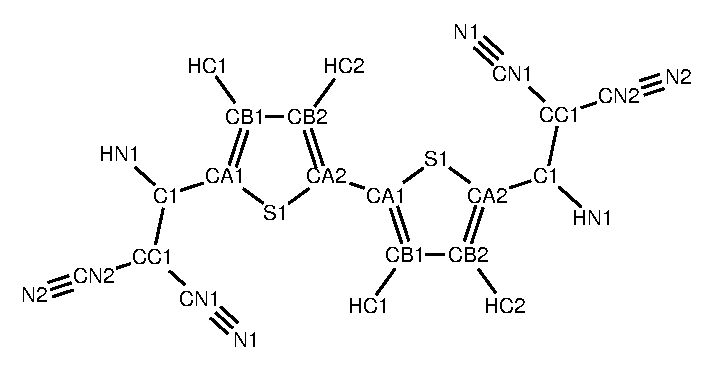
\includegraphics[width=\linewidth]{./fig/chemical_structure/dcv2t_atom_types}
\caption{\small Atom types of DCV2T. The molecule has two types of building blocks (residues), thiophene (THI) and dicyanovinyl (NIT). }
\label{fig:dcv2t_at}
\end{wrapfigure}

%\clearpage
The structure of DCV2T, together with atom type definitions, is shown in fig.~\ref{fig:dcv2t_at}. DCV2T is a typical donor-acceptor-type molecule, with two electron-donating thiophene and two electron-withdrawing dicyanovinyl groups. The pdb file which contains residue types, residue numbering, atom names, atom types, and atom coordinates is shown below. There are two residue types, THI, and NIT, for the thiophene and dicyanovinyl groups, respectively. In its ground state the molecule is practically planar. 

\VerbatimInput[%
frame=lines,
framesep=4mm,
label=\fbox{pdb file of DCV2T}, 
framerule=0.5mm,
rulecolor=\color{red},
baselinestretch=1,
fontsize=\footnotesize%,
%numbers=left
]%
{./fig/chemical_structure/dcv2t.pdb}


\section{Large-scale morphology}
\chapter{Hopping sites}
\label{sec:mapping}

\section{Conjugated segments and rigid fragments}
\label{sec:conjugated_segments}

\begin{wrapfigure}{ht}{0.5\linewidth}
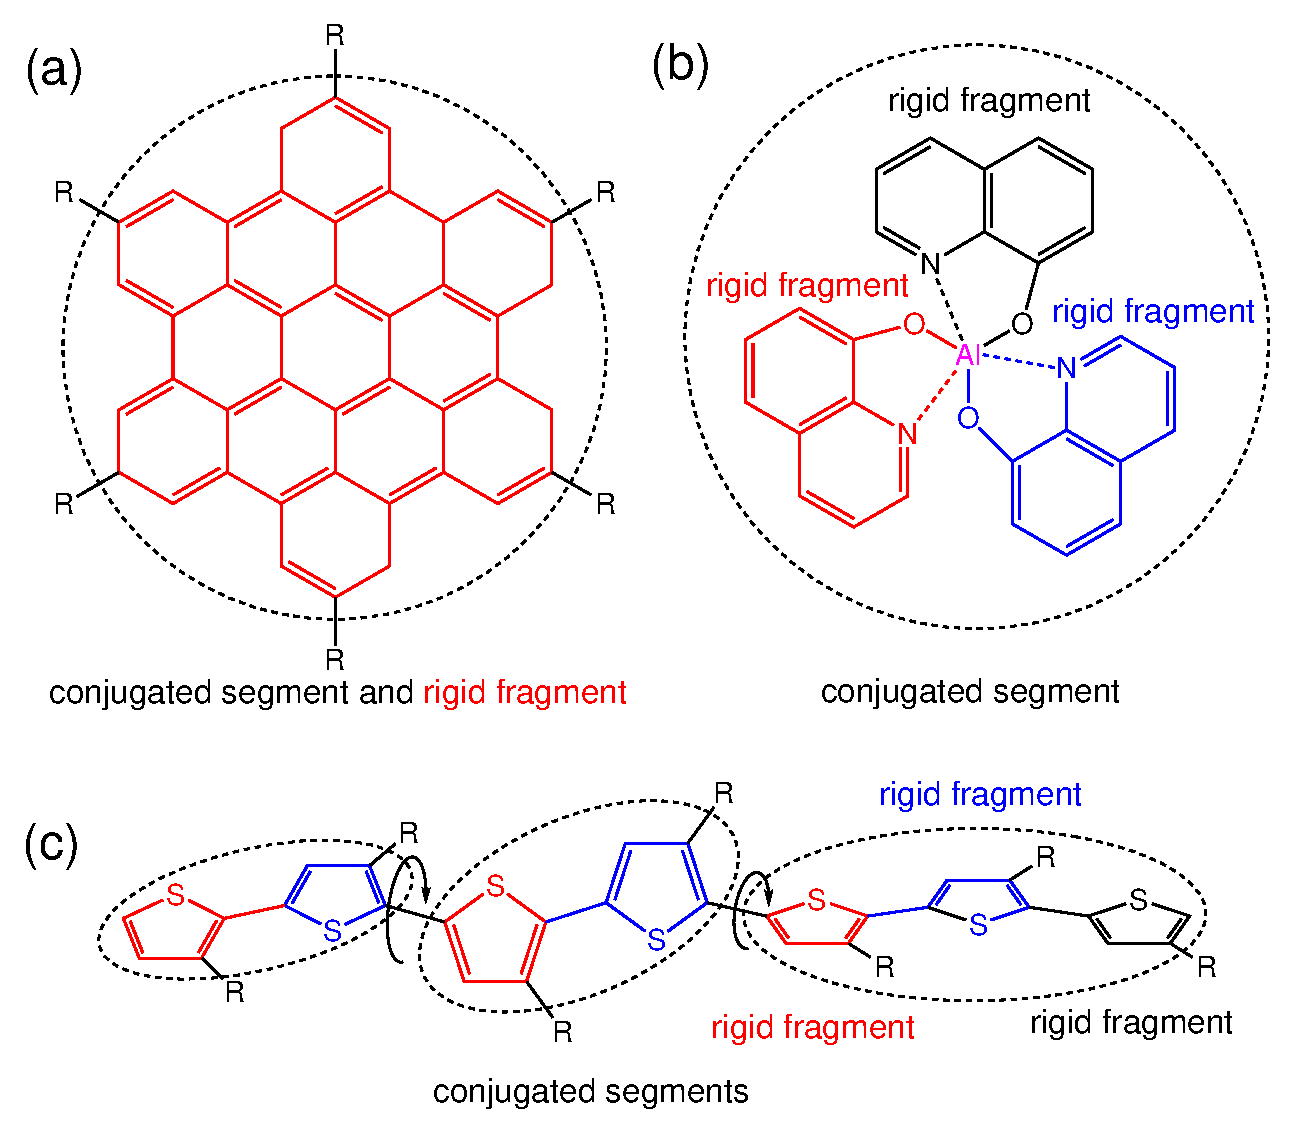
\includegraphics[width=\linewidth]{fig/conjugated_segment/fragment_segment}
\caption{\small The concept of conjugated segments and rigid fragments. Dashed lines indicate conjugated segments while colors denote rigid fragments. (a) Hexabenzocoronene: the $\pi$-conjugated system is both a rigid fragment and a conjugated segment. (b) \Alq: the Al atom and each ligand are rigid fragments while the whole molecule is a conjugated segment. (c) Polythiophene: each repeat unit is a rigid fragment. A conjugated segment consists of one or more rigid fragments. One molecule can have several conjugated segments.}
\label{fig:segment}
\end{wrapfigure}

With the morphology at hand, the next step is partitioning the system on hopping sites, or conjugated segments, and calculating charge transfer rates between them. Physically intuitive arguments can be used for the partitioning,  which reflects the localization of the wave function of a charge. For most organic semiconductors, the molecular architecture includes relatively rigid, planar $\pi$-conjugated systems, which we will refer to as rigid fragments. A conjugated segment can contain one or more of such rigid fragments, which are linked by bonded degrees of freedom. The dynamics of these degrees of freedom evolves on timescales much slower than the frequency of the internal promoting mode. In some cases, e.g. glasses, it can be `frozen' due to non-bonded interactions with the surrounding molecules.

To illustrate the concept of conjugated segments and rigid fragments, three representative molecular architectures are shown in \fig{segment}. The first one is a typical discotic liquid crystal, hexabenzocoronene. It consists of a conjugated core to which side chains are attached to aid self-assembly and solution processing. In this case the orbitals localized on side chains do not participate in charge transport and the conjugated $\pi$-system is both, a rigid fragment and a conjugated segment. 
%
In \Alq, a metal-coordinated compound, a charge carrier is delocalized over all three ligands. Hence, the whole molecule is one conjugated segment. Individual ligands are relatively rigid, while energies of the order of $k_\text{B}T$ are sufficient to reorient them with respect to each other. Thus the Al atom and the three ligands are rigid fragments.
%
In the case of a conjugated polymer, one molecule can consist of several conjugated segments, while each backbone repeat unit is a rigid fragment. Since the conjugation along the backbone can be broken due to large out-of-plane twists between two repeat units, an empirical criterion, based on the dihedral angle, can be used to partition the backbone on conjugated segments~\cite{ruehle_multiscale_2010}. However, such intuitive partitioning is, to some extent, arbitrary and shall be validated by other methods~\cite{vukmirovi_charge_2008,vukmirovi_charge_2009,mcmahon_ad_2009}. 

After partitioning, an additional step is often required to remove bond length fluctuations introduced by molecular dynamics simulations, since they are already integrated out in the derivation of the rate expression. This is achieved by substituting respective molecular fragments with  rigid, planar $\pi$-systems optimized using first-principles methods. Centers of mass and gyration tensors are used to align rigid fragments, though a custom definition of local axes is also possible. Such a procedure also minimizes discrepancies between the force-field and first-principles-based ground state geometries of conjugated segments, which might be important for calculations of electronic couplings, reorganization energies, and intramolecular driving forces. 

Finally, a list of neighboring conjugated segments is constructed. Two segments are added to this list if the distance between centers of mass of {\em any} their rigid fragments is below a certain cutoff. This allows neighbors to be selected on a criterion of minimum distance of approach rather than center of mass distance, which is useful for molecules with anisotropic shapes.

\section{Mapping the system onto conjugated segments}

\texttt{ctp\_map} partitions the system on conjugated segments and rigid fragments
\begin{verbatim}
  ctp_map --top topology.tpr -c 15 -cg cgmap.xml --trj traj.trr
\end{verbatim}
The input are the gromacs topology and trajectory files, a mapping file, a cutoff distance for defining nearest neighbours and a file describing the charge unit types. 

\subsection{The mapping file}
To partition the system onto conjugated segments and rigid fragments a mapping \xml file is required. This file is based on the input provided for generation of \texttt{topol.tpr} and \texttt{traj.trr} files. An example of a mapping file for a single \dcvt molecule is shown in listing~\ref{list:map}.

%\begin{table}
{\small 
\begin{tabular}{p{3cm} p{10cm}}
\xml tag & Description \\
\hline
\texttt{name} & Name of the molecule in the coarse-grained model. Useful for multicomponent systems. \\
%
\texttt{ident} & Name (identification) of the molecule in the all-atom representation. This \emph{must} match the molecule name in the atomistic representation (e.g. \gromacs topology). \\
%
\texttt{topology} & Section describing the partitioning of the molecule on rigid fragments (beads). Atom and residue names/types \emph{must} correspond to those used in the atomistic representation (e.g. \gromacs topology)\\
& \\
\texttt{cg\_beads} & Section describing the different coarse-grained beads (rigid fragments) a molecule or polymer chain may consist of. \\
%
\texttt{cg\_bead} & Section defining one particular bead. \\
%
\texttt{cg\_bead.name} &  The name of the bead. This must be unique for each bead in a molecule. So a polymer made of 10 repeat units needs 10 different bead name identifiers. \\
%
\texttt{cg\_bead.type} &  The type of the bead. This may be the same for beads which only differ by a hydrogen atom or two to simplify the interactions, while the mapping must take such tiny differences into account. \\
%
\texttt{cg\_bead.mapping} & The type of the mapping. Different beads may have the same mapping, since a molecule may contain multiple beads of the same type, but in the bead definition each must correspond to different atoms. \\
%
\texttt{cg\_bead.beads} &  Precise mapping. Lists the molecule labels used in \emph{Gromacs} which form the bead. Note: The first three atoms are used to calculate vectors defining the orientation of the molecule so they must not lie on the same axis. Also the first three atoms in the mapping need not correspond to the first three in the \emph{rtp} or \emph{gro} file, but this mapping must be consistent with the definitions in the list\_charges definition. \\
%
\texttt{cg\_bead.symmetry} &  The symmetry of the molecule. 3 = ellipsoidal with three different axes. \\
& \\
\texttt{qm} & This section associates beads (rigid fragments) with a particular charge unit type \\
%
\texttt{qm.crgunitname} &  The name of the charge unit type the fragment is associated with \\
%
\texttt{qm.bead} & The position of the fragment in the charge unit type. \\
& \\
\texttt{maps} & Section describing the different mapping for all types of beads. \\
%
\texttt{map} &  Section defining one particular map (used to determine the center of a fragment). \\
%
\texttt{map.name} & The name of the mapping. Must correspond to a name used to define the beads above. \\
%
\texttt{map.weights} & The weighting of the atoms inside the bead, usually taken to be the mass of the nucleus in atomic mass units. The weights must be in the same order as the corresponding bead definition.
\end{tabular}
}
%\end{table}

\clearpage

\definecolor{gray}{rgb}{0.4,0.4,0.4}
\definecolor{darkblue}{rgb}{0.0,0.0,0.6}
\definecolor{cyan}{rgb}{0.0,0.6,0.6}

\lstset{
  language=XML,
  frame=lines,
  basicstyle=\ttfamily\footnotesize,
  identifierstyle=\color{red},
  keywordstyle=\color{blue},
  showstringspaces=false,
  columns=fullflexible,
  commentstyle=\color{gray}\rmfamily\itshape,
  morekeywords={cg_molecule,cg_beads,cg_bead,crgunitname,bead,beads,type,topology,name,ident,maps,map,mapping,weights,position,qm,symmetry},
}

\lstinputlisting[
 label=list:map, 
 morekeywords={cg_molecule,cg_beads,name,ident,maps,map,mapping,weights,qm,symmetry},
 caption={Partitioning of DCV2T on conjugates segments and rigid fragments}]%
{./fig/mapping/cgmap.xml}


\chapter{Transfer Integrals}
\label{sec:transfer_integrals}

\subsection{Semi-empirical methods}
\label{sec:moo}

\newcommand{\moo}{MOO\xspace}
\index{electronic coupling!ZINDO}

An approximate method based on Zerner's Independent Neglect of Differential Overlap (ZINDO) has been described in Ref.~\cite{kirkpatrick_approximate_2008}. This semiempirical method is substantially faster than first-principles approaches, since it avoids the self-consistent calculations on each individual monomer and dimer. This allows to construct the matrix elements of the ZINDO Hamiltonian of the dimer from the weighted overlap of molecular orbitals of the two monomers. Together with the introduction of rigid segments, only a single self-consistent calculation on one isolated conjugated segment is required. All relevant molecular overlaps can then be constructed from the obtained molecular orbitals. This Molecular Orbital Overlap (MOO) method has been applied successfully to study charge transport, for instance, in discotic liquid crystals~\cite{kirkpatrick_columnar_2008,marcon_understanding_2009,feng_towards_2009},
polymers~\cite{ruehle_multiscale_2010}, or partially disordered organic crystals~\cite{vehoff_charge_2010-1,vehoff_charge_2010-2,vehoff_charge_2010}.

The main advantage of the molecular orbital overlap \moo library is {\em fast} evaluation of electronic coupling elements. A detailed description of the method is provided in ref.~\cite{kirkpatrick_approximate_2008}. Please site this paper if you are using the method. Note that \moo is based on the semi-empirical ZINDO Hamiltonian and therefore has limited applicability. The general advice is to first compare the accuracy of the \moo method to the DFT-based calculations. 

\moo can be used both in a sandalone mode and as a \calculator of the \votcactp. \moo constructs the Fock operator of a dimer from the  molecular orbitals of monomers by translating and rotating the orbitals and therefore requires the optimized geometry of the molecule and the projection coefficients of the molecular on atomic orbitals. 


\subsubsection{Standalone mode}
For a standalone mode program \overlap is provided 
\begin{verbatim}
 moo_overlap --conjseg benzene.xml --pos1 benzene1.pos --pos2 benzene2.pos
\end{verbatim}
Its input requires a description of two conjugated segments (\texttt{benzene.xml}, positions and orientations of the molecules and the files with molecular coordinates and orbitals. The structure of the files is shown in listings \ref{list:benzene_xml} and  \ref{list:benzene_pos}.
\vskip 0.1cm
\lstinputlisting[
  language=XML,
  label=list:benzene_xml,
  stringstyle=\ttfamily\footnotesize,
  showstringspaces=false,
  caption={\small \texttt{benzene.xml} file with the description of the benzene molecule, which is also a single conjugated segment and a rigid fragment.}] {./programs/benzene.xml}

\vskip 0.1cm

\lstinputlisting[
  language=XML,
  label=list:benzene_pos, 
  stringstyle=\ttfamily\footnotesize,
  showstringspaces=false,
  caption={\small \texttt{benzene1.pos} file which describes the position and orientation of the molecule. The name of the molecule is followed by three coordinates (relative to the center of mass of the supplied \texttt{xyz} file and then by nine elements of the rotation matrix $a_{ij} = e_i e^\text{mol}_j $. The reference coordinate frame is determined from the provided \texttt{xyz} file.}] {./fig/moo/moo_overlap/benzene1.pos}


\subsubsection{Calculator of \votcactp}
Semi-empirical method of evaluation of electronic couplings in a morphology is provided by the \integrals \calculator. In addition to definitions of conjugated segments, atomistic trajectory, and state file, the program needs coordinates and orbitals of conjugated segments. Coordinates are stored in \xyz files with four columns, first being the atom type and the next three atom coordinates. This is a standard \texttt{xyz} format without a header. Note that the atom order in \xyz files can be different from that of the mapping files. The correspondence between the two is established in the file which defines conjugated segments.

\section{Density-functional}
\begin{itemize}
\item {\it not sure about directory structure yet, using {\tt
      \$DIRECTORY} for the time being}
\item creating file structure for frame $N$ (raw: no postpocessing,
  min: MD energy minimization) in directory {\tt OUTDIR}
\begin{verbatim}
$DIRECTORY/perpare.sh raw/min N OUTDIR
cd OUTDIR
$DIRECTORY/pairdump.sh
\end{verbatim}
\item make sure QCP environments are set!
\item running calculations for all monomers
 \begin{verbatim}
$DIRECTORY/calc_monomer QCP [METHOD]

QCP:   G for Gaussian09
       T for Turbomole

METHOD: func/basis (optional)
        overrides default functional/basisset combination
        defaults: pbepbe/6-311G** Gaussian09
                  b-p/def-TZVP    Turbomole
\end{verbatim}
\item check monomer calculations (Gaussian version to test!) 
\begin{verbatim}
$DIRECTORY/check_mols N M QCP

N:   First monomer to test
M:   Last monomer to test
QCP: G/T 
\end{verbatim}
incomplete monomers are written to file {\tt TROUBLE.mol}
\item running calculations for all dimers
 \begin{verbatim}
$DIRECTORY/calc_dimer_noSCF QCP [METHOD]

QCP:   G for Gaussian09
       T for Turbomole

METHOD: func/basis (optional)
        overrides default functional/basisset combination
        defaults: pbepbe/6-311G** Gaussian09
                  b-p/def-TZVP    Turbomole
\end{verbatim}
\item should we add {\tt trajectory\_submit.sh} that does all monomer
  and dimer calculations on the cluster (MPIP-specific)?
\end{itemize}



\chapter{Site energies}
\label{sec:site_energies}

\newcommand{\estat}{\hyperref[calc:estat]{\texttt{estat}}\xspace}

\section{Electrostatic energy}
\label{sec:electrostatic}
Variations of the local electric field can result in large electrostatic contributions to the energetic disorder. Using the atomic partial charges of charged and neutral molecules, $\Delta E_{ij}^\text{el}$ can be computed from the site energies~\cite{kirkpatrick_columnar_2008}
\begin{equation}
E_{i}^\text{el}  = \frac{1}{4 \pi \epsilon_0} \sum_{a_i} \sum_{\substack{b_k   \\ k\neq i }}
\frac{ \left( q^c_{a_i} - q^n_{a_i} \right) q^n_{b_k}}{ \epsilon_\text{s} r_{a_i b_k}} 
\, ,
\label{equ:estatic}
\end{equation}
where $r_{a_i b_k}=|\vec{r}_{a_i} - \vec{r}_{b_k}|$ is the distance between atoms $a_i$ and $b_k$,   $\epsilon_\text{s}$ is the static relative dielectric constant.
%
The first sum extends over all atoms of molecule $i$, for which the site energy is calculated. The second sum reflects interactions with all atoms of neutral molecules $k \ne i$. By using \equ{estatic}, one assumes that the influence of conformational changes on partial charges and changes of the molecular geometry upon charging are small. In order to minimize finite size effects, we do not use spherical cutoff but apply the nearest image convention, that is sum over all neutral molecules in the box after centering the box around the charged molecule. 

The influence of polarization effects on the Coulomb interactions can be taken into account by using a relative dielectric constant in \equ{estatic}. Bulk values of  $\epsilon_\text{s} = 2-5$ for typical organic semiconductors uniformly scale all site energies but are not capable of describing polarization effects on a microscopic level. 
The contribution to $E_i^\text{el}$ from the first coordination shell is then underestimated due to overscreening and, as a result, the site-energy differences become artificially small. Alternatively, one can introduce a phenomenological distance-dependent screening function $\epsilon(r_{a_i b_k})$ in~\equ{estatic}~\cite{nagata_atomistic_2008}
\begin{equation}
\epsilon(r)=\epsilon_{\text{s}} - (\epsilon_{\text{s}} - 1)
\left( 1 + sr + \frac{1}{2}s^2r^2 \right) 
\mathrm{e}^{ -sr}\,,
\label{equ:epss}
\end{equation}
where the parameter $s$ is the inverse screening length. For a monovalent ion in water, for example, $\epsilon_{\text{s}}=80$ and $s=3\,\textrm{nm}^{-1}$~\cite{daggett_molecular_1991}. This screening function ensures that neighboring atoms interact via an unscreened Coulomb potential ($\epsilon \sim 1$) while the electrostatic interaction between atoms at large separations is screened as in the bulk. 

Evaluation of the electrostatic contribution is provided by the \estat calculator of \texttt{ctp\_run} 
\begin{verbatim}
  ctp_run --exec "estat"
\end{verbatim}
\suggestion{Need to describe all possible options, with and without screening, etc}
\section{Master equation}
\label{sec:kmc}
\index{kinetic Monte Carlo}
Having determined the list of conjugated segments (hopping sites) and charge transfer rates between them, the next task is to solve the master equation which describes the time evolution of the system
%
\begin{equation}
\label{equ:master}
\frac{\partial P_\alpha}{\partial t} = \sum_{\beta} P_\beta \Omega_{\beta \alpha} - 
\sum_{\beta} P_\alpha \Omega_{\alpha \beta},
\end{equation}
%
where $P_\alpha$ is the probability of the system to be in a state $\alpha$ at time $t$ and $\Omega_{\alpha \beta}$ is the transition rate from state $\alpha$ to state $\beta$. A state $\alpha$ is specified by a set of site occupations, $\left\{ \alpha_i \right\}$, where $\alpha_i = 1 (0)$ for an occupied (unoccupied) site $i$, and the matrix $\hat{\Omega}$ can be constructed from rates $\omega_{ij}$.

The solution of \equ{master} is be obtained by using kinetic Monte Carlo (KMC) methods. KMC explicitly simulates the dynamics of charge carriers by constructing a Markov chain in state space and can find both stationary and transient solutions of the master equation. The main advantage of KMC is that only states with a direct link to the current state need to be considered at each step. Since these can be constructed solely from current site occupations, extensions to multiple charge carriers (without the mean-field approximation), site-occupation dependent rates (needed for the explicit treatment of Coulomb interactions), and different types of interacting particles and processes, are straightforward. To optimize memory usage and efficiency, a combination of the variable step size method~\cite{bortz_new_1975} and the first reaction method is implemented.

To obtain the dynamics of charges using KMC, the program \kmcrun executes a specific \calculator after reading its options (charge carrier type, runtime, numer of carriers etc.) from \xmloptions. 

\votcacommand{KMC for a single carrier in periodic boundary conditions}{\cmdkmcsin}

\votcacommand{KMC for multiple carriers of the same type in periodic boundary conditions}{\cmdkmc}

\chapter{Manual pages}

\section{Programs}
\label{ref:programs}
\input{reference/programs/all}

\section{Calculators}
\label{ref:caclulators}
\input{reference/calculators/all}

\section{Options}
\label{ref:options}
\input{reference/xml/ctp_listcharges.xml}



\bibliographystyle{achemso}
\bibliography{literature_short}

\end{document} 
